\chapter{Εισαγωγικά στο \tl{MATLAB}}\label{ch:prelim}
Για να κατανοήσουμε και να ελέγξουμε διάφορα πολύπλοκα συστήματα πρέπει να
καταφύγουμε σε κάποιο μαθηματικό μοντέλο των συστημάτων αυτών. Η σύνθεση
του μαθηματικού μοντέλου προκύπτει από τις διαφορικές εξισώσεις που περιγράφουν
τη δυναμική συμπεριφορά του συστήματος. Τα περισσότερα συστήματα παρουσιάζουν
μη-γραμμική συμπεριφορά. Η προσέγγιση που ακολουθούμε στα συστήματα αυτομάτου
ελέγχου περιλαμβάνει τη γραμμικοποίηση των μη-γραμμικών διαφορικών εξισώσεων
γύρω από ένα σημείο ισορροπίας και έτσι λαμβάνεται το αντίστοιχο προσεγγιστικό
γραμμικό μοντέλο. Στη συνέχεια χρησιμοποιείται ο μετασχηματισμός \tl{Laplace}
όπου μετατρέπουμε τις διαφορικές εξισώσεις, από το πεδίο του χρόνου, σε
αλγεβρικές, στο πεδίο της συχνότητας, που λύνονται πολύ πιο εύκολα. Με τη
βοήθεια του μετασχηματισμού καταλήγουμε σε μία σχέση εισόδου-εξόδου
του συστήματος, που καλείται συνάρτηση μεταφοράς. Η συνάρτηση μεταφοράς αποτελεί
ένα μέσο για τη μελέτη της συμπεριφοράς του συστήματος για διάφορα σήματα
εισόδου που επιδρούν στο σύστημα. Για περισσότερες πληροφορίες για τα θέματα του
αυτομάτου ελέγχου προτείνονται τα βιβλία~\cite{dorf2011modern}
και~\cite{ogata2011modern}.

\section{Συναρτήσεις μεταφοράς}
Η συνάρτηση μεταφοράς είναι της μορφής
\[
    G(s) = \frac{Y(s)}{U(s)},
\]
όπου \( Y(s) \) και \( U(s) \) είναι οι μετασχηματισμοί \tl{Laplace} των
χρονικών συναρτήσεων εξόδου και εισόδου αντίστοιχα. Γενικά τα συστήματα ελέγχου
είναι ιδιαίτερα πολύπλοκα, για και η μελέτη τους γίνεται με εξειδικευμένα
λογισμικά, όπως το \tl{MATLAB}. Στη συνέχεια θα παρουσιάσουμε βασικές εντολές
του \tl{MATLAB} για τη δημιουργία, την ανάλυση και την παρουσίαση συστημάτων
ελέγχου. Αυτό θα γίνει με τη μορφή παραδειγμάτων και την παράθεση του
αντίστοιχου κώδικα και την επεξήγηση αυτού.

Η δημιουργία συνάρτησης μεταφοράς στο \tl{MATLAB} γίνεται με την εντολή
\mono{tf} και συντάσσεται
\eng{
    \begin{center}
        sys = tf(num, den)
    \end{center}
}
όπου οι είσοδοι της συνάρτησης είναι οι πίνακες \mono{num} και \mono{den}, που
δηλώνουν τα πολυώνυμα του αριθμητή και παρανομαστή αντίστοιχα και η έξοδος
\mono{sys} είναι η συνάρτηση μεταφοράς. Οι εντολές για τη δήλωση των παραπάνω
στο \tl{MATLAB} φαίνονται παρακάτω.
\eng{\lstinputlisting[language=Matlab]{src/prelim1.m}}

Μία άλλη χρήσιμη δυνατότητα είναι η γρήγορη εύρεση των μηδενικών και των πόλων
του συστήματος. Μηδενικά ονομάζονται οι όροι που μηδενίζουν τον αριθμητή της
συνάρτησης μεταφοράς και πόλοι οι όροι που μηδενίζουν τον παρανομαστή. Είναι
γνωστό ότι αν πόλοι βρίσκονται στο αριστερό ημιεπίπεδο τότε το σύστημα είναι
ευσταθές. Μιας και ασχολούμαστε με γραμμικά συστήματα, η ευστάθεια είναι
του συστήματος είναι ανεξάρτητη της διέγερσης. Με την εντολή \mono{pzmap(sys)}
θα δημιουργηθεί διάγραμμα με τον άξονα \( x \) να είναι ο άξονας των
πραγματικών αριθμών και τον άξονα \( y \) να είναι ο άξονας των φανταστικών
αριθμών. Ένα τέτοιο παράδειγμα είναι το εξής.
\eng{\lstinputlisting[language=Matlab]{src/prelim2.m}}
\begin{figure}[h]
    \centering
    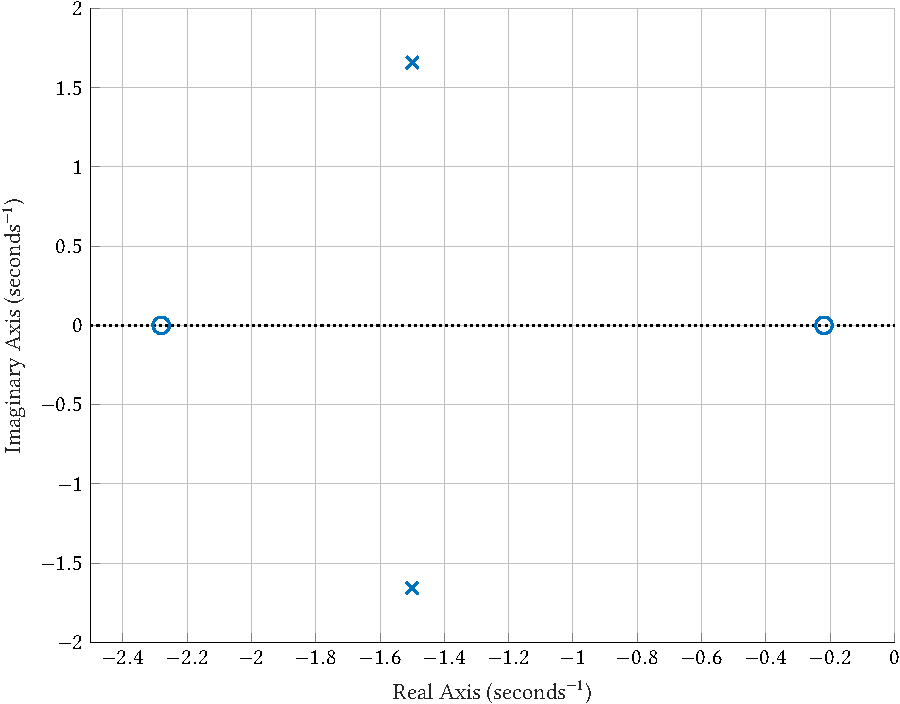
\includegraphics[width=0.9\textwidth]{figures/prelim2.pdf}
    \captionG{Διάγραμμα πόλων-μηδενικών, (\( o \) μηδενικά, \( x \) πόλοι)}
    \label{fig:prelim2}
\end{figure}
Το διάγραμμα που παίρνουμε φαίνεται στο σχήμα~\ref{fig:prelim2}. Οι πόλοι
συμβολίζονται με το σύμβολο \( x \) και τα μηδενικά με το σύμβολο \( o \).
Βλέπουμε πως οι πόλοι βρίσκονται στο αριστερό ημιεπίπεδο και άρα το σύστημα είναι ευσταθές.

Με το \tl{MATLAB} μπορούμε να δηλώσουμε ένα σύστημα κλειστού βρόχου με την
εντολή \mono{feedback}. Με την ανάδραση σε ένα σύστημα κλειστού βρόχου μπορούμε
να συγκρίνουμε την έξοδο του συστήματος με την είσοδο του συστήματος, έτσι ώστε
η επιθυμητή δράση ελέγχου να αποτελεί συνάρτηση της εξόδου και της εισόδου του
συστήματος. Η σύνταξη στο \tl{MATLAB} είναι
\eng{
    \begin{center}
        sys = feedback(sys1, sys2)
    \end{center}
}
όπου \mono{sys1} είναι η συνάρτηση μεταφοράς του ανοιχτού βρόχου και \mono{sys2}
είναι συνάρτηση μεταφοράς του κλάδου της ανάδρασης. Αξίζει να σημειωθεί ότι από
προεπιλογή η εντολή \mono{feedback} θεωρεί αρνητική ανάδραση. Φυσικά έχουμε την
επιλογή να αλλάξουμε τη συμπεριφορά αυτή αν το επιθυμούμε. Για περαιτέρω ο
ενδιαφερόμενος παραπέμπεται στη βοήθεια του \tl{MATLAB}. Στη συνέχεια
παρουσιάζεται παράδειγμα με τις απαραίτητες εντολές, που έχει συνάρτηση μεταφοράς
\[
    G(s) = \frac{4}{s^2 + 2s + 3},
\]
και θέλουμε μοναδιαία ανάδραση.
\eng{\lstinputlisting[language=Matlab]{src/prelim3.m}}

Αν το σύστημα που πρόκειται να ελέγξουμε είναι μη-γραμμικό ή χρονικά
μεταβαλλόμενο ή έχει πολλαπλές εισόδους και εξόδους τότε είναι δύσκολο, αν όχι
αδύνατον, να εξαχθεί η συνάρτηση μεταφοράς του μοντέλου. Για αυτόν το λόγο
χρησιμοποιούμε το μοντέλο μεταβλητών κατάστασης για να περιγράψουμε το σύστημα.

Σύμφωνα με το βιβλίο~\cite{lin2007robust}, το μοντέλο μεταβλητών κατάστασης ενός
συστήματος ορίζεται ως ο ελάχιστος αριθμός μεταβλητών, όπου η γνώση των οποίων
σε οποιοδήποτε χρόνο σε συνδυασμό με την πληροφορία της εισόδου που εφαρμόζεται
στο χρόνο αυτό, είναι ικανή συνθήκη για να προσδιορίσουμε την κατάσταση του
συστήματος για κάθε μελλοντικό χρόνο. Συνήθως χρησιμοποιούμε ένα διάνυσμα
διάστασης \( n \) για να συμβολίσουμε τις μεταβλητές κατάστασης, \( x \in
\mathbb{R}^n \).  Χρησιμοποιούμε το διάνυσμα \( u \in \mathbb{R}^m \) για να
συμβολίσουμε τις \( m \) μεταβλητές εισόδου και \( y \in \mathbb{R}^p \) για να
συμβολίσουμε τις \( p \) μεταβλητές εξόδου. Η γενική μορφή ενός μοντέλου στο
χώρο των καταστάσεων είναι της μορφής
\begin{align*}
    \dot{x} &= f(x, u, t) \\
    y &= g(x, u, t).
\end{align*}
Στην περίπτωση που οι συναρτήσεις \( f, g \) είναι ανεξάρτητες του χρόνου
\( t \) αλλά είναι και γραμμικές, τότε το μοντέλο μεταβλητών κατάστασης
γράφεται στη μορφή
\begin{align}\label{eq:prelim_ss}
    \dot{x} &= Ax + Bu\nonumber \\
    y &= Cx + Du.
\end{align}

Η δημιουργία μοντέλου μεταβλητών κατάστασης στο \tl{MATLAB} γίνεται με την
εντολή \mono{ss}.
\eng{
    \begin{center}
        sys = ss(A, B, C, D)
    \end{center}
}
Οι είσοδοι της συνάρτησης είναι οι πίνακες \( A, B, C, D \), όπως φαίνονται
στις σχέσεις~\eqref{eq:prelim_ss}. Παρακάτω παρατίθεται ένα παράδειγμα με τις
αντίστοιχες εντολές του \tl{MATLAB}.
\eng{\lstinputlisting[language=Matlab]{src/prelim4.m}}

\section{Απόκριση συστήματος}
Μπορούμε να διερευνήσουμε την απόκριση του συστήματος στο πεδίο του χρόνου
χρησιμοποιώντας στη συνάρτηση \mono{step}. Η συνάρτηση αυτή είναι από τις πιο
χρήσιμες συναρτήσεις του \tl{MATLAB} για το σχεδιασμό συστημάτων ελέγχου.
Δοθέντος ενός συστήματος, λαμβάνουμε την απόκριση σε μοναδιαία είσοδο, χωρίς την
ανάγκη να λύσουμε ως προς το χρόνο το σύστημα. Η συνάρτηση \mono{step} μπορεί να
περιγράφει ως η αλλαγή στην είσοδο από το μηδέν στο ένα στο χρόνο ένα. Η σύνταξη
είναι
\eng{
    \begin{center}
        step(sys)
    \end{center}
}
όπου \mono{sys} είναι δυναμικό σύστημα, για παράδειγμα θα μπορούσε να είναι
κάποιο από τα παραπάνω παραδείγματα. Αν πάρουμε για παράδειγμα ένα σύστημα
δεύτερης τάξης
\[
    G(s) = \frac{\omega_n^2}{s^2 + 2\zeta\omega_n + \omega_n^2},
\]
με \( \omega_n = 1 \) και \( \zeta = 0.25 \) και τρέξουμε τις ακόλουθες εντολές
στο \tl{MATLAB} θα λάβουμε το σχήμα~\ref{fig:prelim5}.
\eng{\lstinputlisting[language=Matlab]{src/prelim5.m}}
\begin{figure}[h!]
    \centering
    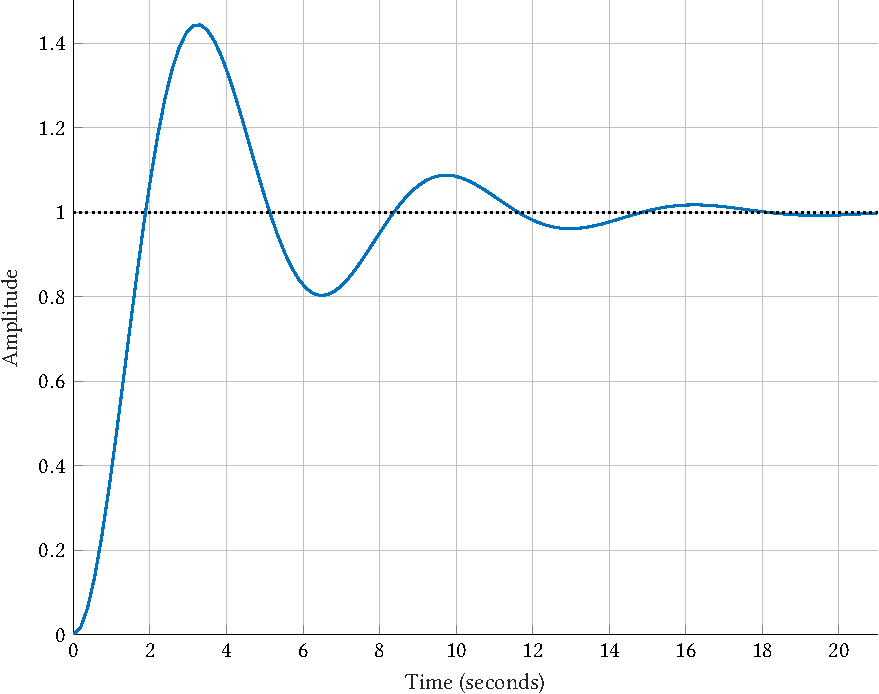
\includegraphics[width=0.9\textwidth]{figures/prelim5.pdf}
    \captionG{Μοναδιαία βηματική απόκριση}
    \label{fig:prelim5}
\end{figure}
Η απόκριση του συστήματος ανοιχτού βρόχου, είναι η αναμενόμενη διότι η απόσβεση
είναι μικρή και έτσι έχουμε ταλαντώσεις αλλά και αργή σύγκλιση.

\begin{figure}[h!]
    \centering
    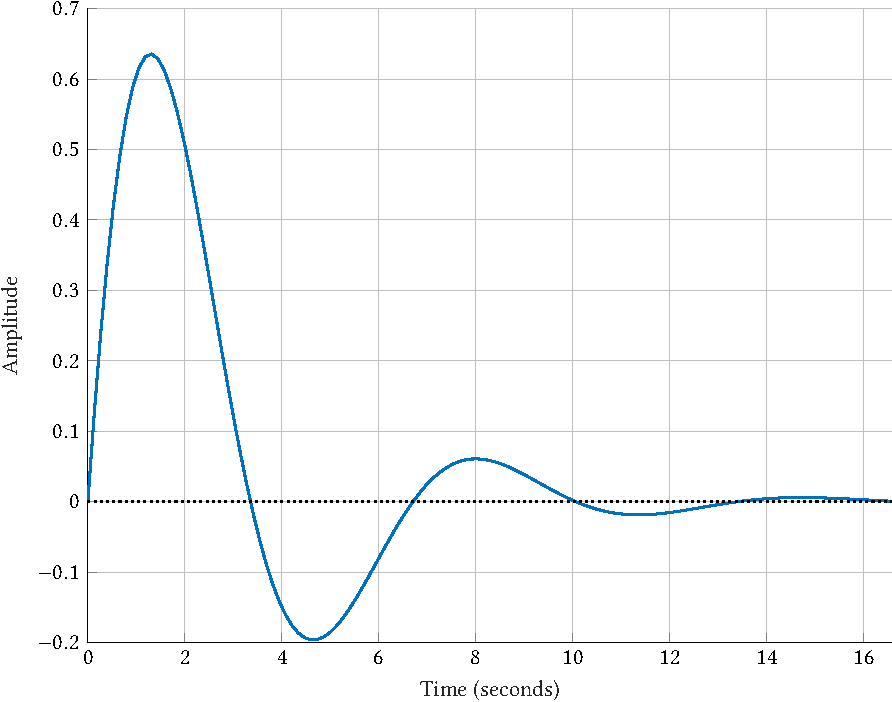
\includegraphics[width=0.9\textwidth]{figures/prelim6.pdf}
    \captionG{Κρουστική απόκριση}
    \label{fig:prelim6}
\end{figure}
Ένα άλλο εργαλείο που μας παρέχει το \tl{MATLAB} για τη διερεύνηση της απόκρισης
του συστήματος είναι η συνάρτηση \mono{impulse}. Η συνάρτηση αυτή υπολογίζει την
απόκριση του συστήματος που υπόκειται σε κρουστική είσοδο, δηλαδή στη συνάρτηση
\( \delta(t) \) του \tl{Dirac}. Η σύνταξη είναι όμοια με αυτή της \mono{step}
που παρουσιάσαμε παραπάνω. Παρακάτω παρουσιάζονται οι εντολές του \tl{MATLAB}
για την απόκριση του προηγούμενου παραδείγματος, αλλά με \( \zeta = 0.7 \)
σε κρουστική είσοδο και η συμπεριφορά του συστήματος εμφανίζεται στο
σχήμα~\ref{fig:prelim6}. Παρατηρούμε πως η συγκεκριμένη τιμή του \( \zeta \) μας
δίνει καλύτερα δυναμικά χαρακτηριστικά, δηλαδή μικρότερες ταλαντώσεις και
γρηγορότερη σύγκλιση στη μόνιμη κατάσταση.
\eng{\lstinputlisting[language=Matlab]{src/prelim6.m}}

Εκτός από τις συναρτήσεις \mono{step} και \mono{impulse} έχουμε τη δυνατότητα να
μελετήσουμε την απόκριση του συστήματος για οποιοδήποτε σήμα εισόδου επιθυμούμε.
Αυτό γίνεται με τη συνάρτηση \mono{lsim} που συντάσσεται
\eng{
    \begin{center}
        lsim(sys, u, t)
    \end{center}
}
όπου \mono{sys} είναι το σύστημα, \mono{u} είναι συνάρτηση της εισόδου που
επιθυμούμε και \mono{t} είναι ο χρονικός ορίζοντας. Σαν παράδειγμα μπορούμε να
δούμε πως ανταποκρίνεται ένα σύστημα δεύτερης τάξης σε
\enquote*{τετραγωνικό} σήμα.
\eng{\lstinputlisting[language=Matlab]{src/prelim7.m}}
Στο παράδειγμα έχουμε φυσική συχνότητα \( \omega_n = 1 \), συντελεστή
απόσβεσης \( \zeta = 0.77 \) και τετραγωνικό σήμα εισόδου.
\begin{figure}[h]
    \centering
    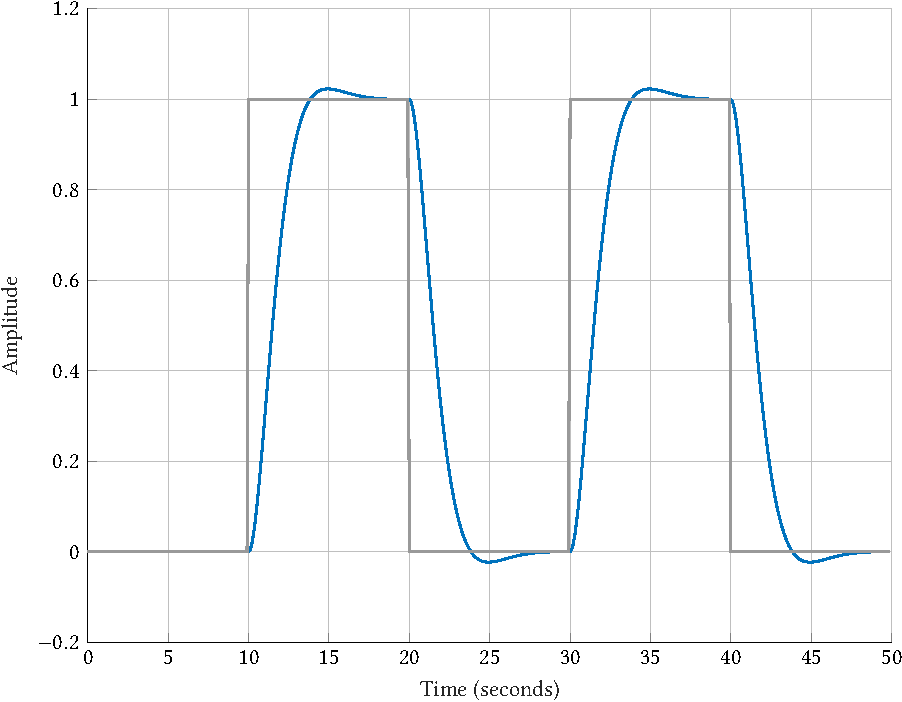
\includegraphics[width=0.9\textwidth]{figures/prelim7.pdf}
    \captionG{\gr{Απόκριση σε τετραγωνικό σήμα εισόδου}}
    \label{fig:prelim7}
\end{figure}
Στο σχήμα~\ref{fig:prelim7}, με τη μπλε γραμμή εμφανίζεται η απόκριση του
συστήματος και με τη γκρι το σήμα εισόδου, δηλαδή η επιθυμητή τροχιά. Με τη
συνάρτηση \mono{gensig} μπορούμε να δημιουργήσουμε διάφορα σήματα εισόδου.
Φυσικά όμως έχουμε τη δυνατότητα να ορίσουμε οπουδήποτε συνάρτηση
εισόδου \( u \) επιθυμούμε και να τη χρησιμοποιήσουμε με την \mono{lsim}.

\section{Επίλυση συστημάτων βέλτιστου ελέγχου}
Τέλος, με τη βοήθεια του \tl{MATLAB} είναι πολύ εύκολη η επίλυση συστημάτων
βέλτιστου ελέγχου. Με την εντολή
\eng{
    \begin{center}
        [K, S, e] = lqr(A, B, Q, R, N)
    \end{center}
}
υπολογίζουμε το βέλτιστο νόμο ελέγχου \( K \). Πιο συγκεκριμένα, για ένα σύστημα
ελέγχου συνεχούς χρόνου, ο βέλτιστος νόμος ελέγχου \( u = -Kx \) είναι αυτός που
ελαχιστοποιεί την τετραγωνική αντικειμενική συνάρτηση
\[
    J = \int_0^{\infty} \left( x^TQx + u^TRu + 2x^TNu \right) ,\ dt
\]
όπου \( Q, R \) είναι τα μητρώα στάθμισης των μεταβλητών κατάστασης και των
μεταβλητών ελέγχου και \( N \) είναι το μητρώο στάθμισης των μεταβλητών
κατάστασης συναρτήσει των μεταβλητών ελέγχου. Η ελαχιστοποίηση της παραπάνω
γίνεται δεδομένου ότι ικανοποιούνται οι εξισώσεις της δυναμικής του συστήματος
\[
    \dot{x} = Ax + Bu.
\]
Τελικά, καταλήγουμε στην αλγεβρική εξίσωση \tl{Riccati}
\[
    A^T + SA - (SB + N)R^{-1}(B^TS + N^T) + Q = 0,
\]
της οποίας τη λύση βρίσκουμε με την εντολή \mono{lqr}. Σαν παράδειγμα θα δούμε
το σύστημα μεταβλητών κατάστασης που είδαμε σε προηγούμενο παράδειγμα. Οι
ιδιοτιμές του μητρώου \( A \) είναι \( \lambda_1 = -1, \lambda_2 = 2 \)
και συνεπώς είναι ασταθές. Με τις παρακάτω εντολές κατασκευάζουμε βέλτιστο
ελεγκτή με μοναδιαία στάθμιση στις μεταβλητές κατάστασης \( Q = I_2 \),
στάθμιση στη μεταβλητή εισόδου \( R = 10 \) και \( N = 0 \).
\eng{\lstinputlisting[language=Matlab]{src/prelim8.m}}
Το κέρδος υπολογίζεται
\[
    K = \begin{bmatrix}4.0248 & 4.0248\end{bmatrix},
\]
και η μοναδιαία βηματική απόκριση του βέλτιστου τετραγωνικού ελεγκτή
παρουσιάζεται στο σχήμα~\ref{fig:prelim8}.
\begin{figure}[h]
    \centering
    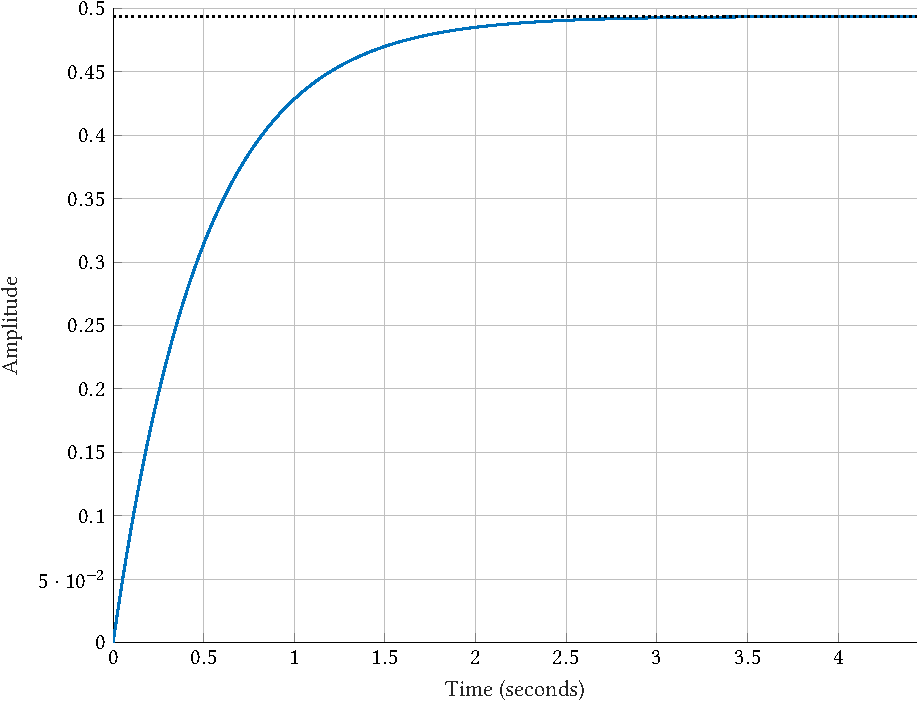
\includegraphics[width=0.9\textwidth]{figures/prelim8.pdf}
    \captionG{Μοναδιαία βηματική απόκριση βέλτιστου τετραγωνικού ελεγκτή}
    \label{fig:prelim8}
\end{figure}
